\documentclass[10pt,a4paper]{article}

\usepackage[margin=0.75in]{geometry}
\usepackage{graphicx}
\usepackage{amsmath}
\usepackage{amssymb}
\usepackage{booktabs}
\usepackage{array}
\usepackage{float}
\usepackage{caption}
\usepackage{subcaption}
\usepackage{xcolor}
\usepackage{hyperref}
\usepackage{multicol}
\usepackage{titlesec}

\definecolor{umtblue}{RGB}{32,63,145}
\hypersetup{colorlinks=true, linkcolor=umtblue, urlcolor=umtblue, citecolor=umtblue}
\titleformat{\section}{\large\bfseries\color{umtblue}}{\thesection}{0.5em}{}
\titleformat{\subsection}{\normalsize\bfseries}{\thesubsection}{0.5em}{}
\captionsetup{font=small, labelfont=bf}

\title{\vspace{-1.2cm}\textbf{Predicting English Premier League Match Results Using Machine Learning}\\
\large CS446 -- Machine Learning, Spring 2026}
\author{Muhammad Owais Saeed\\University of Management and Technology\\Section V2}
\date{}

\begin{document}
\maketitle
\vspace{-0.8cm}

\begin{abstract}
Predicting football match outcomes is a challenging classification task because match results depend on historical performance, team form, home advantage, and random in-game events. This project applies supervised machine learning algorithms to predict English Premier League (EPL) match outcomes as Home Win, Draw, or Away Win. Historical match data from seasons 2000--01 to 2017--18 was used, with engineered features such as team points, goal difference, recent form, win streaks, loss streaks, and normalized cumulative statistics. Five classifiers were implemented: K-Nearest Neighbors, Logistic Regression, Gaussian Naive Bayes, Support Vector Machine with RBF kernel, and Neural Network. The best trained classifier was SVM, achieving an accuracy of 51.58\% on the test set. Bet365 odds were also evaluated as a test-only benchmark and achieved 54.56\% accuracy. Results show that machine learning models can outperform a random baseline but still struggle strongly with draw prediction.
\end{abstract}

\section{Introduction and Problem Statement}
Football analytics has become an important area in sports data science. Clubs, analysts, and betting markets are interested in predicting match results using historical statistics. The English Premier League is highly competitive, and its results are difficult to predict due to uncertainty, tactical variation, injuries, player form, and home-ground effects.

The objective of this project is to formulate EPL match prediction as a three-class supervised classification problem. For each match, the model predicts:
\begin{itemize}
    \item Home Win (H),
    \item Draw (D),
    \item Away Win (A).
\end{itemize}
The central problem is to transform historical match statistics into meaningful numerical features and compare the predictive performance of different machine learning classifiers.

\section{Related Work / Literature Review}
Sports prediction has frequently been studied using statistical and machine learning techniques. Traditional approaches include logistic regression and probabilistic models because they are interpretable and work well with tabular data. More advanced classifiers such as support vector machines and neural networks can model nonlinear relationships, but their success depends strongly on feature quality and dataset size.

Previous football prediction studies commonly use team form, goal difference, recent wins, home advantage, and betting odds as explanatory variables. Betting odds are particularly informative because they combine expert knowledge, market behavior, and public information. However, odds should not be used as a normal training feature when they are only available for the test period; therefore, this project treats Bet365 implied probabilities as a separate test-only benchmark.

\section{Methodology}
\subsection{Dataset and Preprocessing}
The dataset consists of EPL season CSV files and a processed \texttt{final\_dataset.csv}. Match outcome labels were recovered using Date, HomeTeam, and AwayTeam keys from the original season files. The target variable was converted into a three-class label: A, D, and H.

Recent form columns were mapped into numerical values:
\[
W=3, \quad D=1, \quad L=0, \quad M=0.
\]
Cumulative statistics such as points and goal difference were normalized by match week to keep feature windows consistent across early and late season matches:
\[
HTP_n = \frac{HTP}{MW}, \quad ATP_n = \frac{ATP}{MW}.
\]
A chronological split was used to avoid future information leakage. The global model was trained on earlier matches and tested on later matches.

\subsection{Feature Extraction}
The selected features include goals scored, goals conceded, normalized points, five-match form, form points, win streaks, loss streaks, normalized goal difference, point difference, and form difference. These features represent both long-term team strength and short-term recent momentum.

\subsection{Models}
Five classifiers were trained and evaluated:
\begin{enumerate}
    \item K-Nearest Neighbors (KNN),
    \item Logistic Regression,
    \item Gaussian Naive Bayes,
    \item Support Vector Machine (RBF kernel),
    \item Multi-Layer Perceptron Neural Network.
\end{enumerate}
All features were standardized using \texttt{StandardScaler} before training.

\section{Mathematical Formulation}
Let each match be represented by a feature vector \(x_i \in \mathbb{R}^{d}\) and a target label \(y_i \in \{A,D,H\}\). The goal is to learn a classifier:
\[
f: \mathbb{R}^{d} \rightarrow \{A,D,H\}.
\]
Accuracy is computed as:
\[
Accuracy = \frac{\text{Number of correct predictions}}{\text{Total predictions}}.
\]
Macro F1 is calculated as the average F1-score across all classes:
\[
F1_{macro}=\frac{1}{3}(F1_A+F1_D+F1_H).
\]
For Logistic Regression, the probability of a class is modeled using a softmax function:
\[
P(y=k|x)=\frac{e^{w_k^Tx+b_k}}{\sum_j e^{w_j^Tx+b_j}}.
\]
For SVM, the RBF kernel is defined as:
\[
K(x_i,x_j)=\exp(-\gamma ||x_i-x_j||^2).
\]

\section{Results and Discussion}
\subsection{Global Test Performance}
Table~\ref{tab:global} shows the global test performance of all trained classifiers. SVM achieved the highest model accuracy.

\begin{table}[H]
\centering
\caption{Global model performance.}
\label{tab:global}
\begin{tabular}{lcc}
\toprule
Classifier & Accuracy & Macro F1 \\
\midrule
KNN & 0.4974 & 0.4191 \\
Logistic Regression & 0.5123 & 0.3744 \\
Naive Bayes & 0.4956 & 0.3927 \\
SVM (RBF) & \textbf{0.5158} & 0.3767 \\
Neural Network & 0.4289 & 0.3965 \\
Bet365 Odds & \textbf{0.5456} & \textbf{0.4044} \\
\bottomrule
\end{tabular}
\end{table}

\begin{figure}[H]
\centering
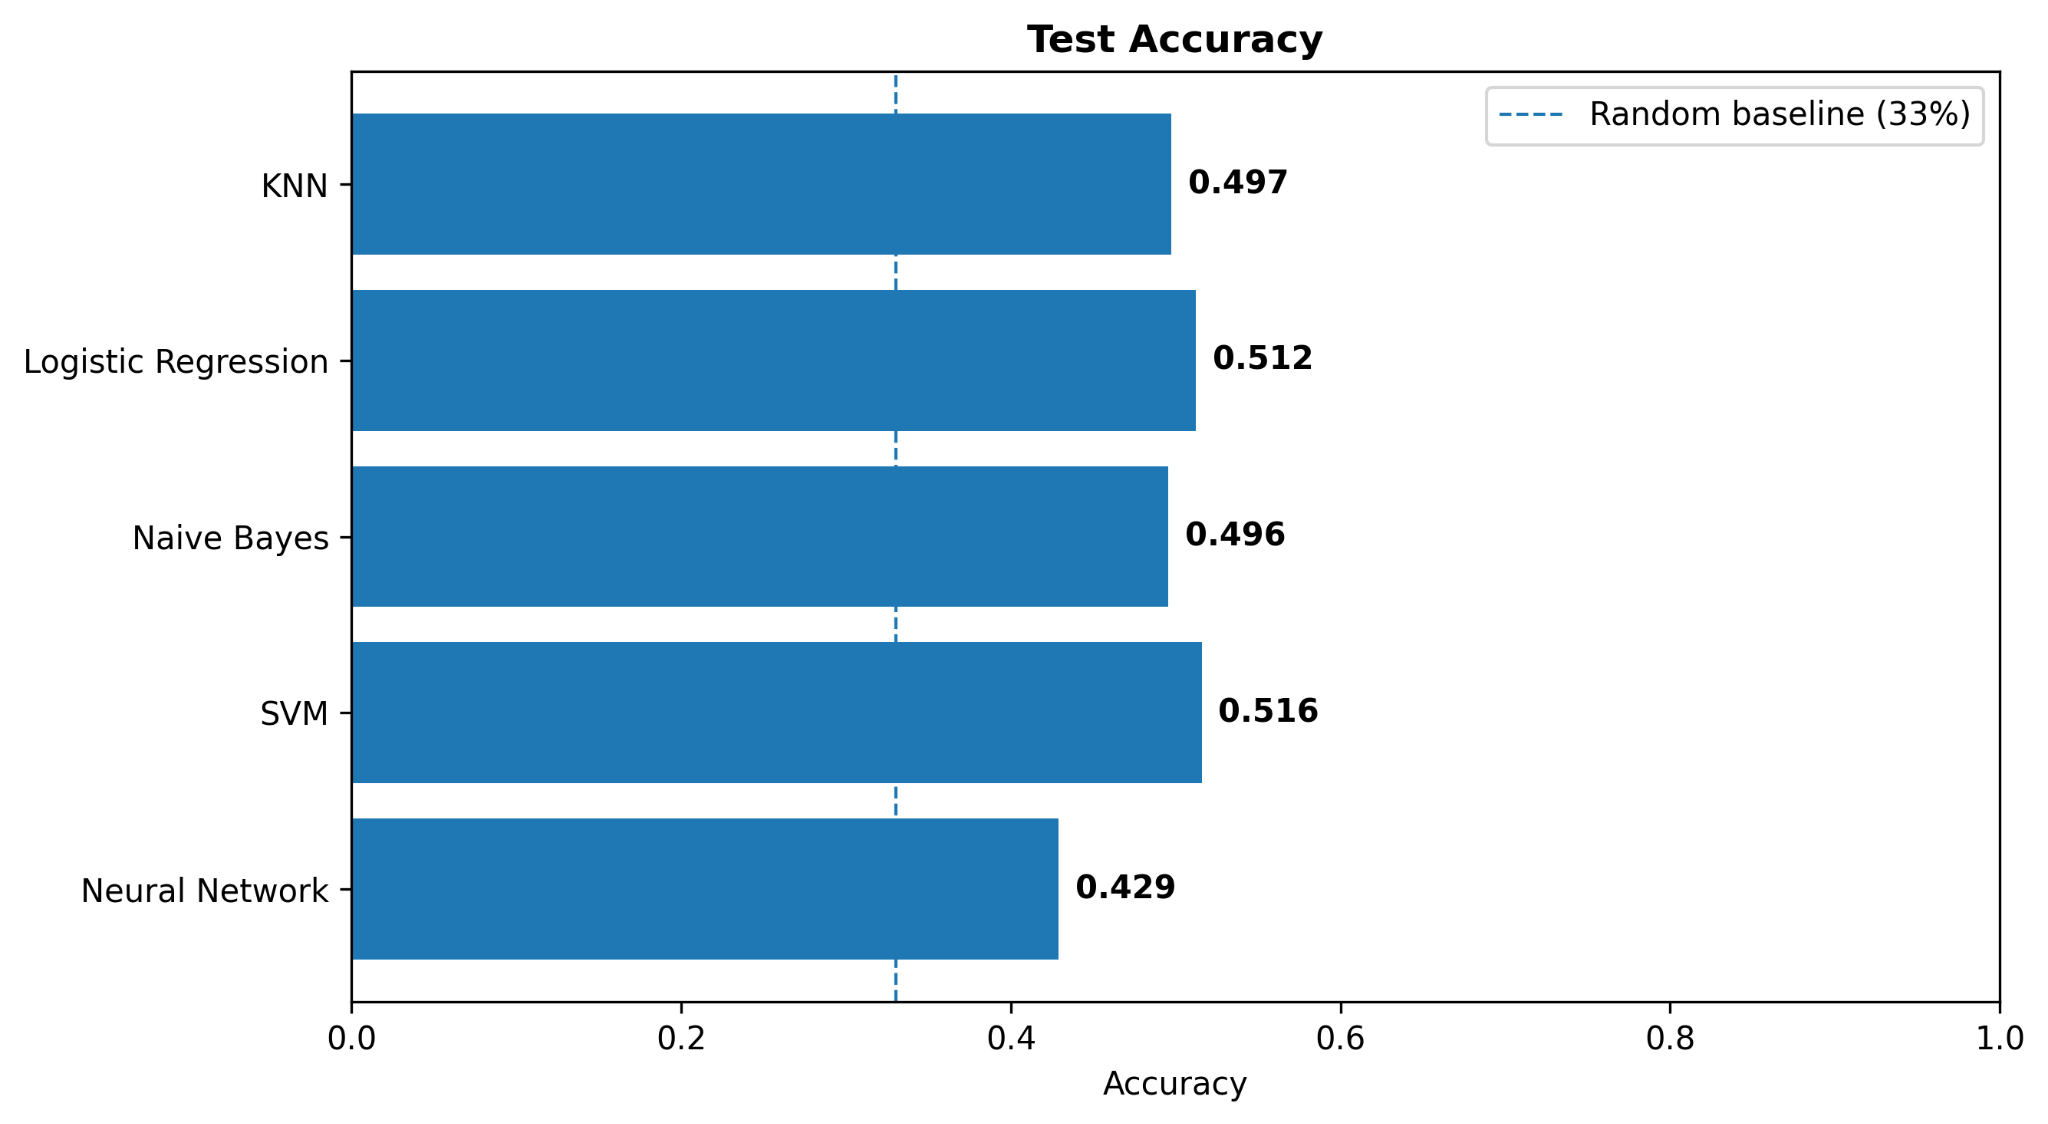
\includegraphics[width=0.82\linewidth]{../figures/01_test_accuracy.png}
\caption{Test accuracy comparison of five classifiers.}
\end{figure}

The SVM model obtained the best trained-classifier accuracy of 51.58\%. Bet365 odds achieved a higher accuracy of 54.56\%, which suggests that bookmaker odds contain information not captured by historical form features alone.

\subsection{Confusion Matrix Analysis}
The confusion matrices show that the classifiers tend to predict Home Win more often than Draw. This is especially visible for SVM, where draw recall is very low. This indicates class imbalance and the natural difficulty of predicting draws.

\begin{figure}[H]
\centering
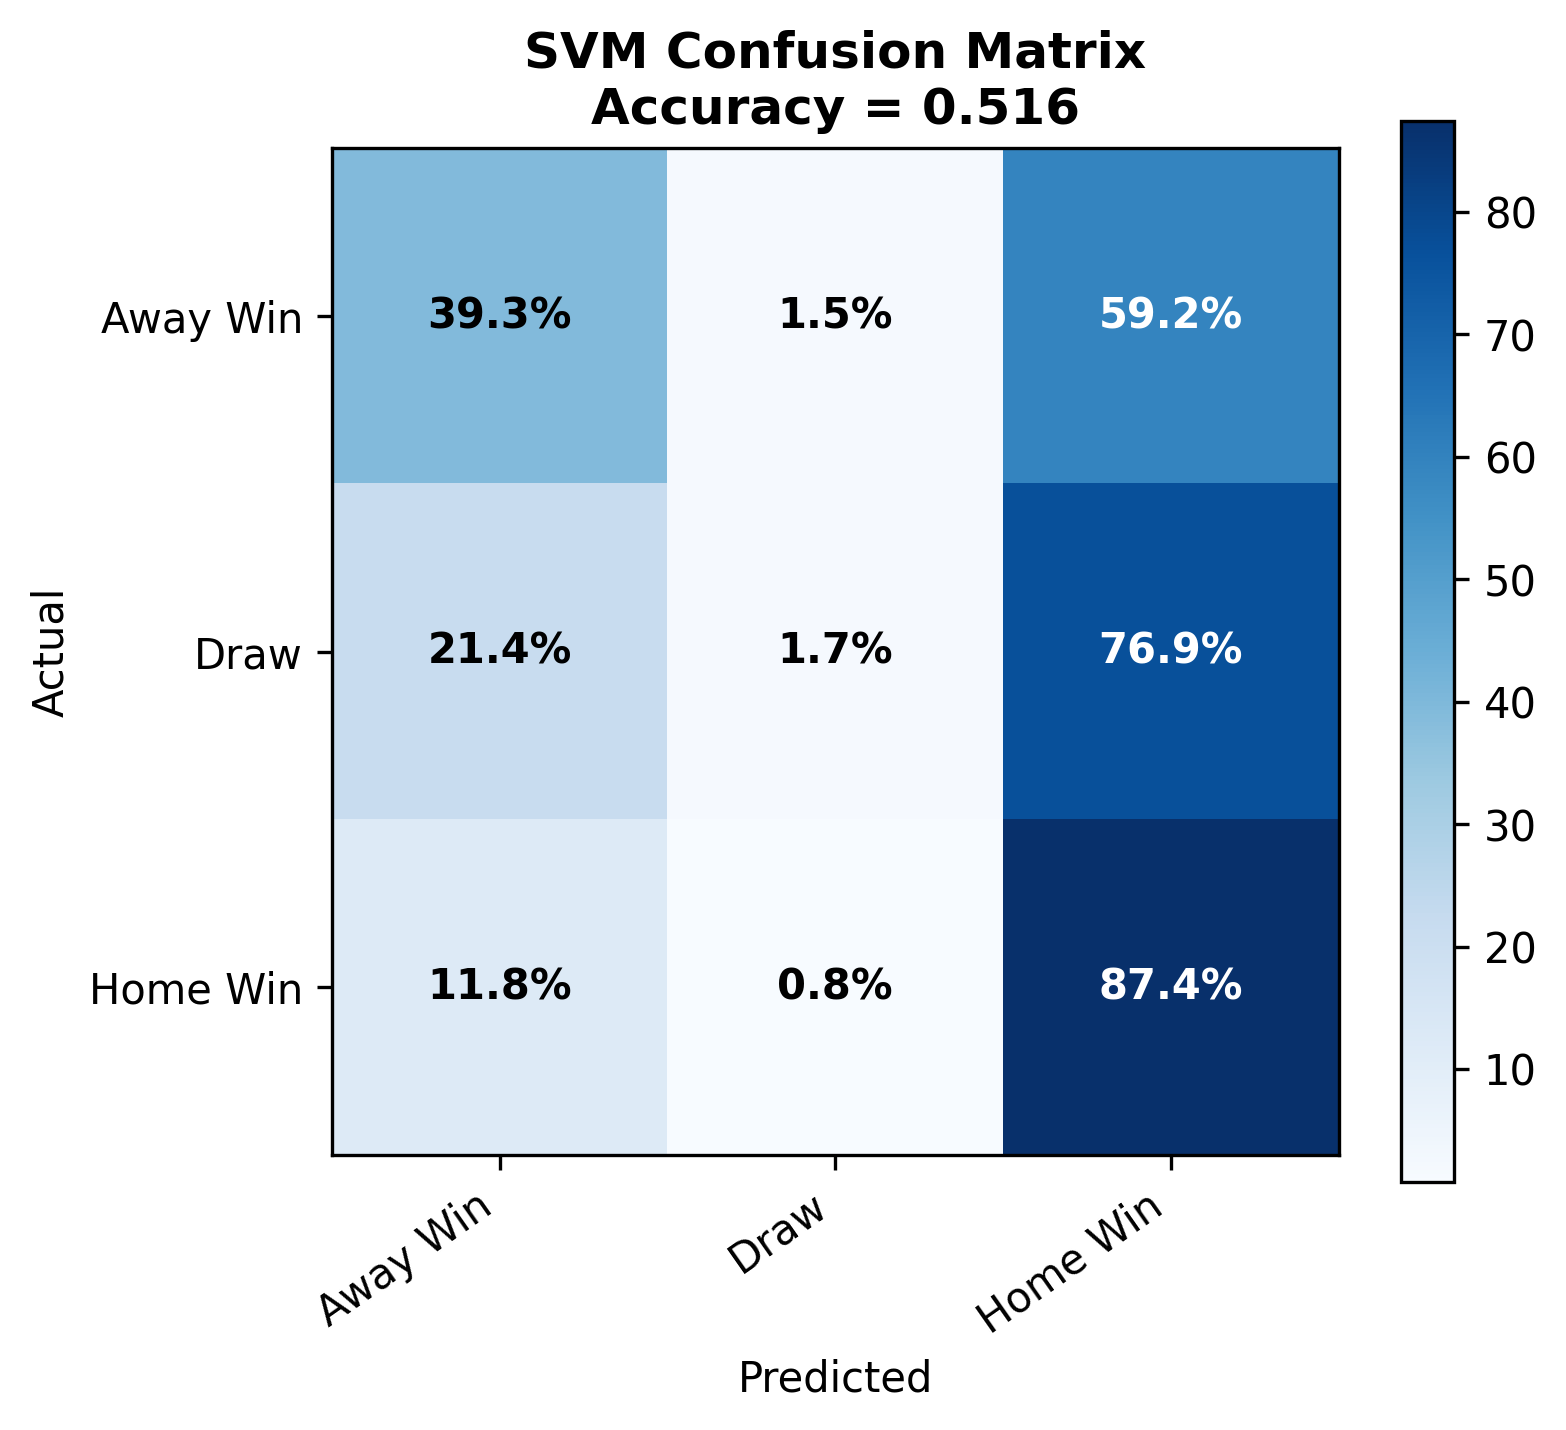
\includegraphics[width=0.55\linewidth]{../figures/02_confusion_matrix_svm.png}
\caption{Confusion matrix of the best trained model: SVM.}
\end{figure}

\begin{figure}[H]
\centering
\begin{subfigure}{0.48\linewidth}
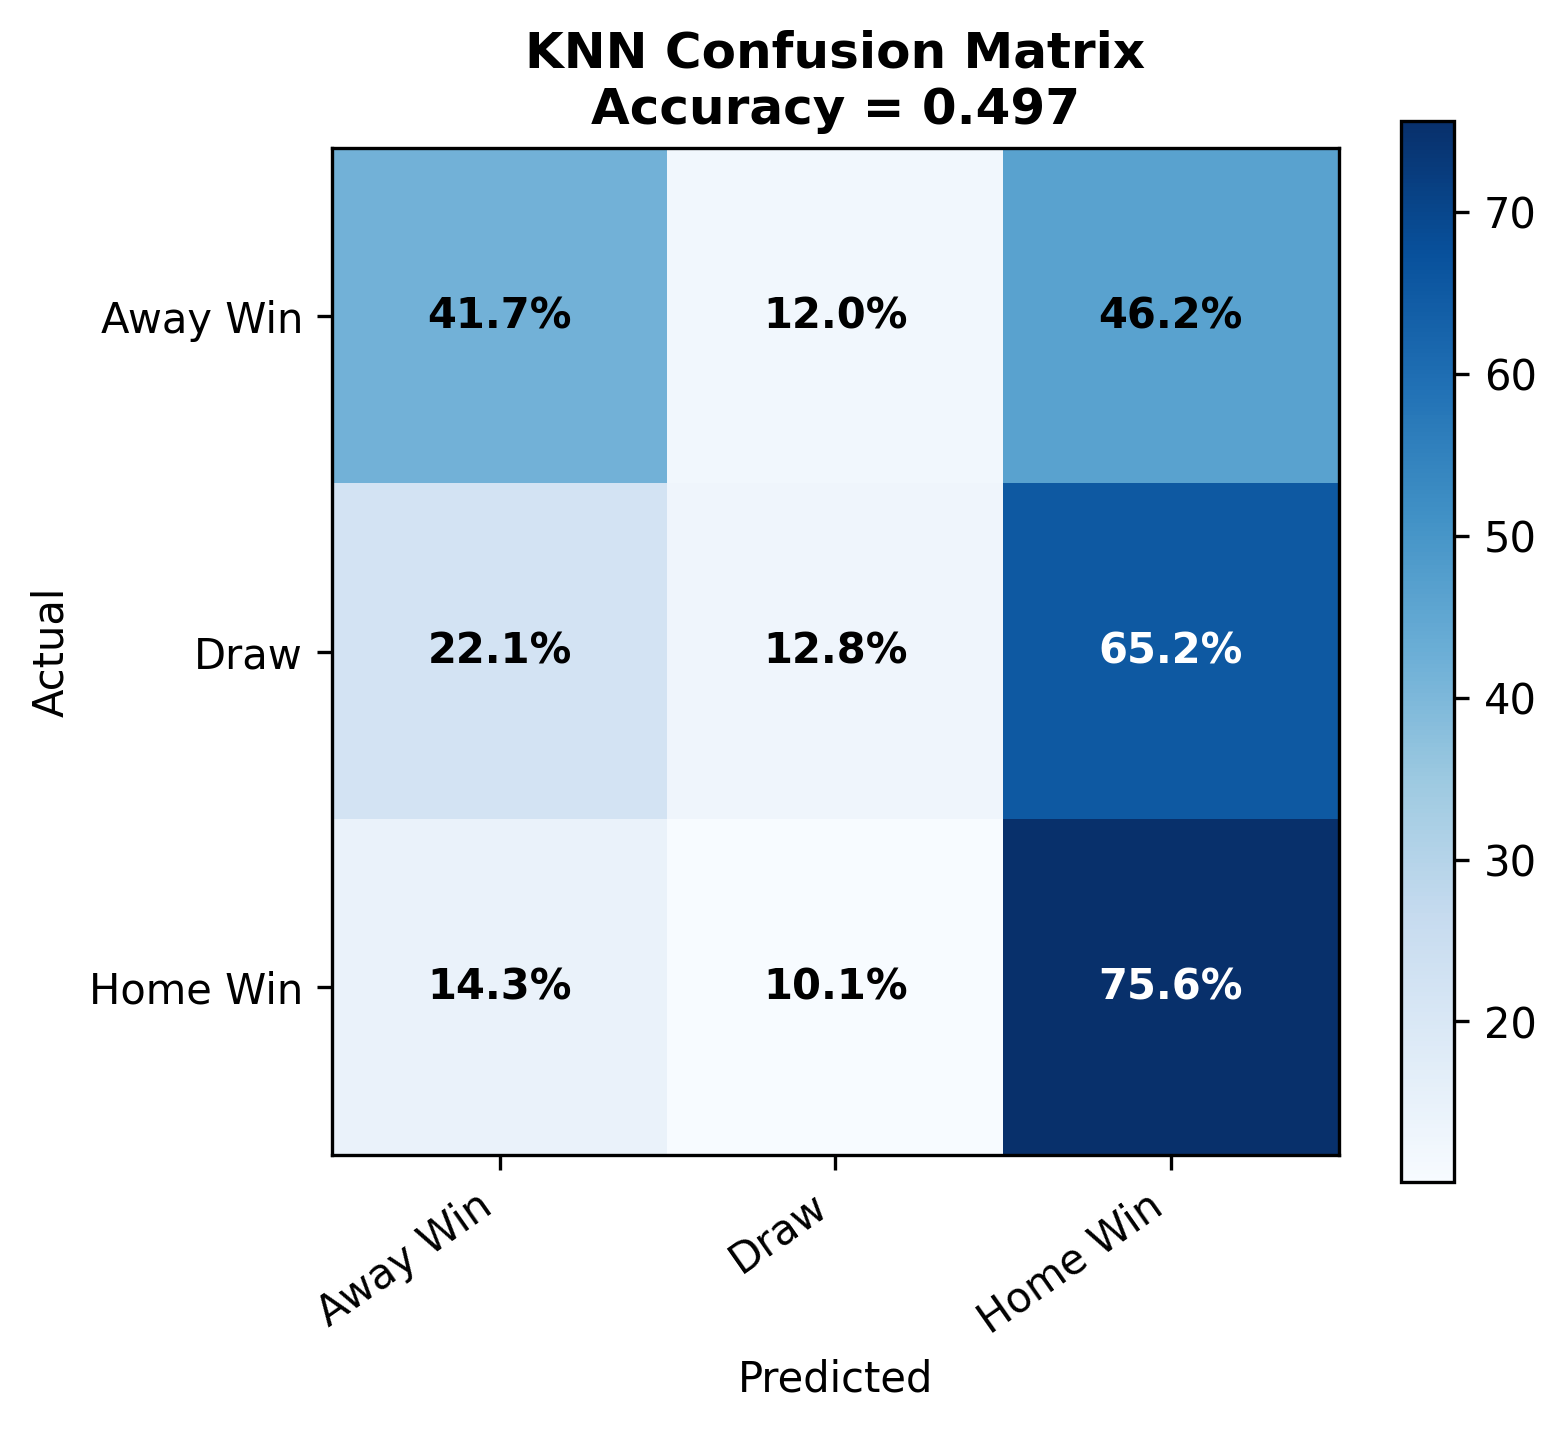
\includegraphics[width=\linewidth]{../figures/02_confusion_matrix_knn.png}
\caption{KNN}
\end{subfigure}
\begin{subfigure}{0.48\linewidth}
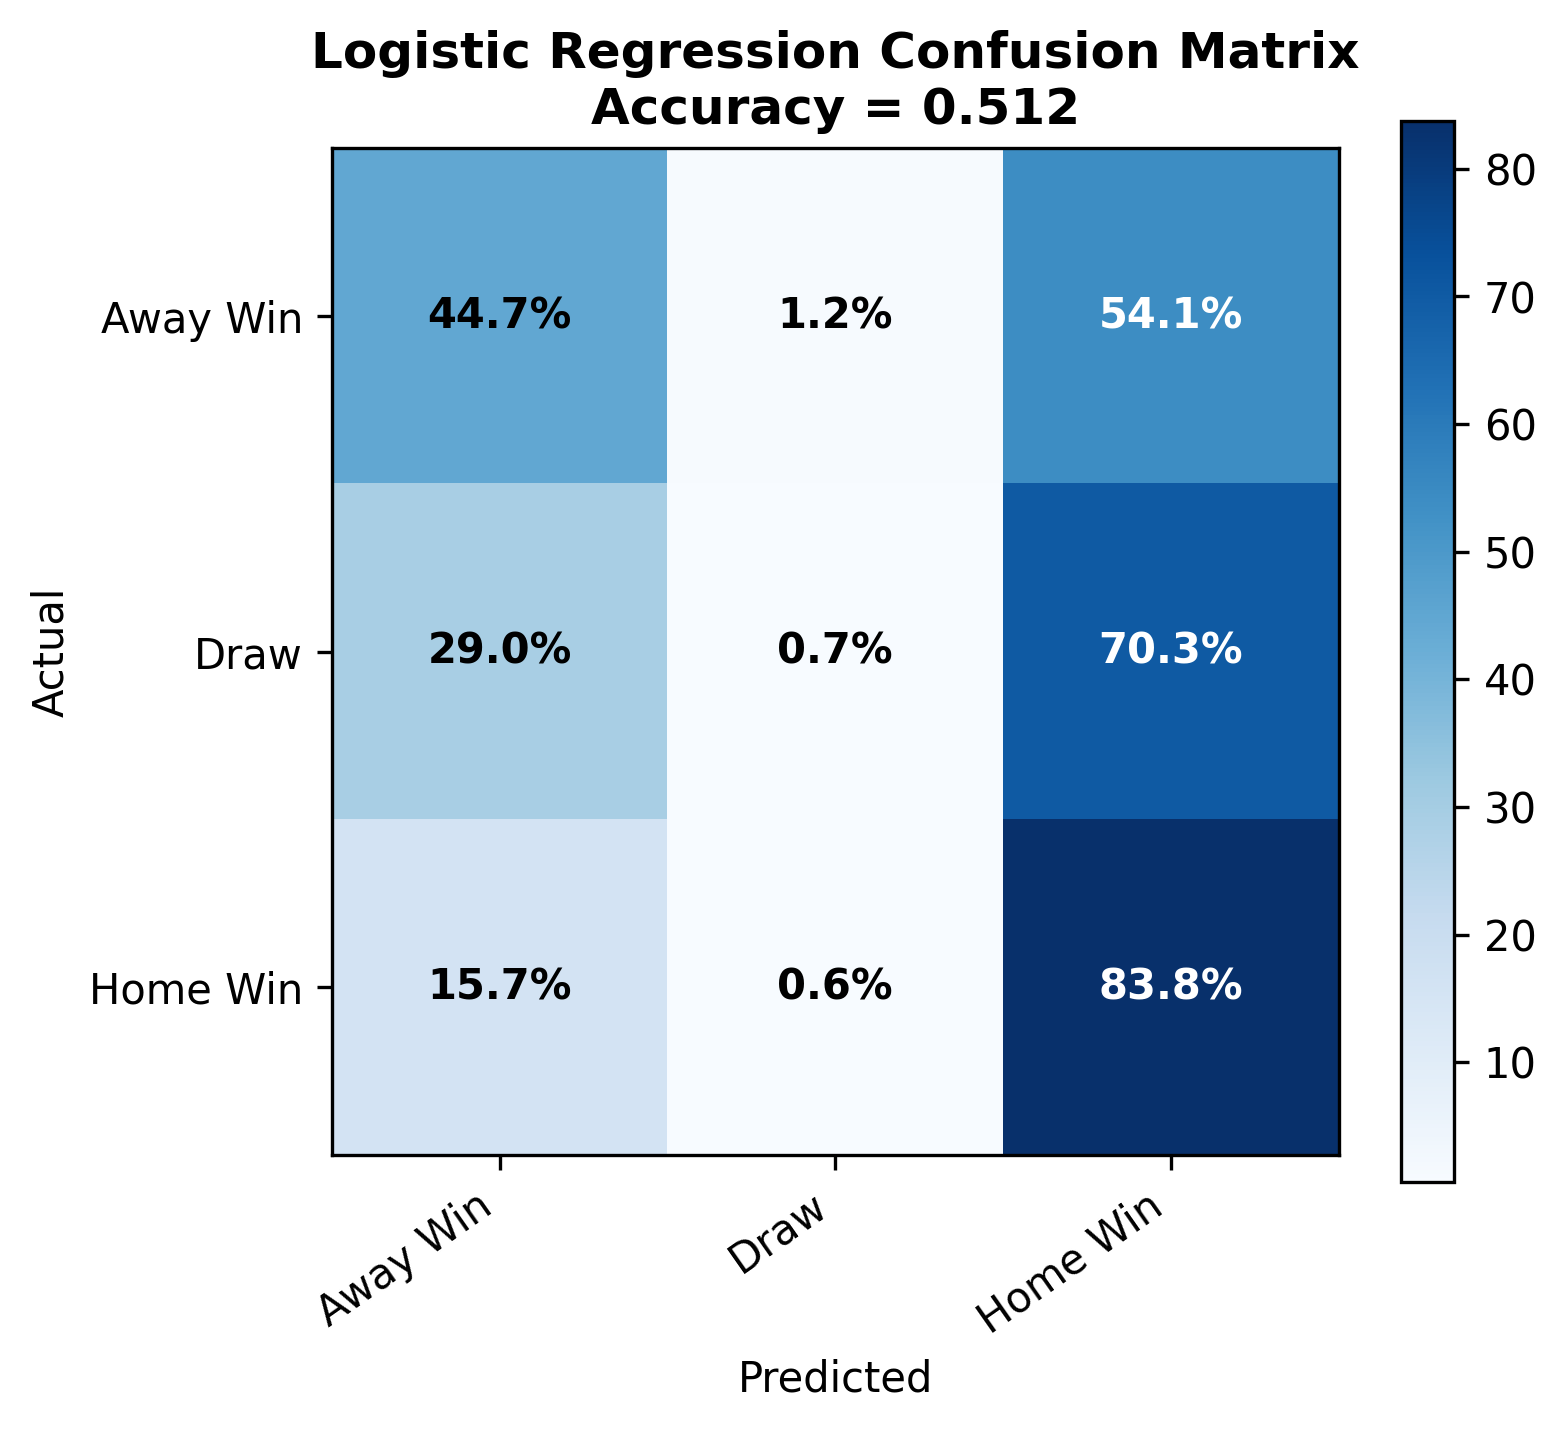
\includegraphics[width=\linewidth]{../figures/02_confusion_matrix_logistic_regression.png}
\caption{Logistic Regression}
\end{subfigure}
\begin{subfigure}{0.48\linewidth}
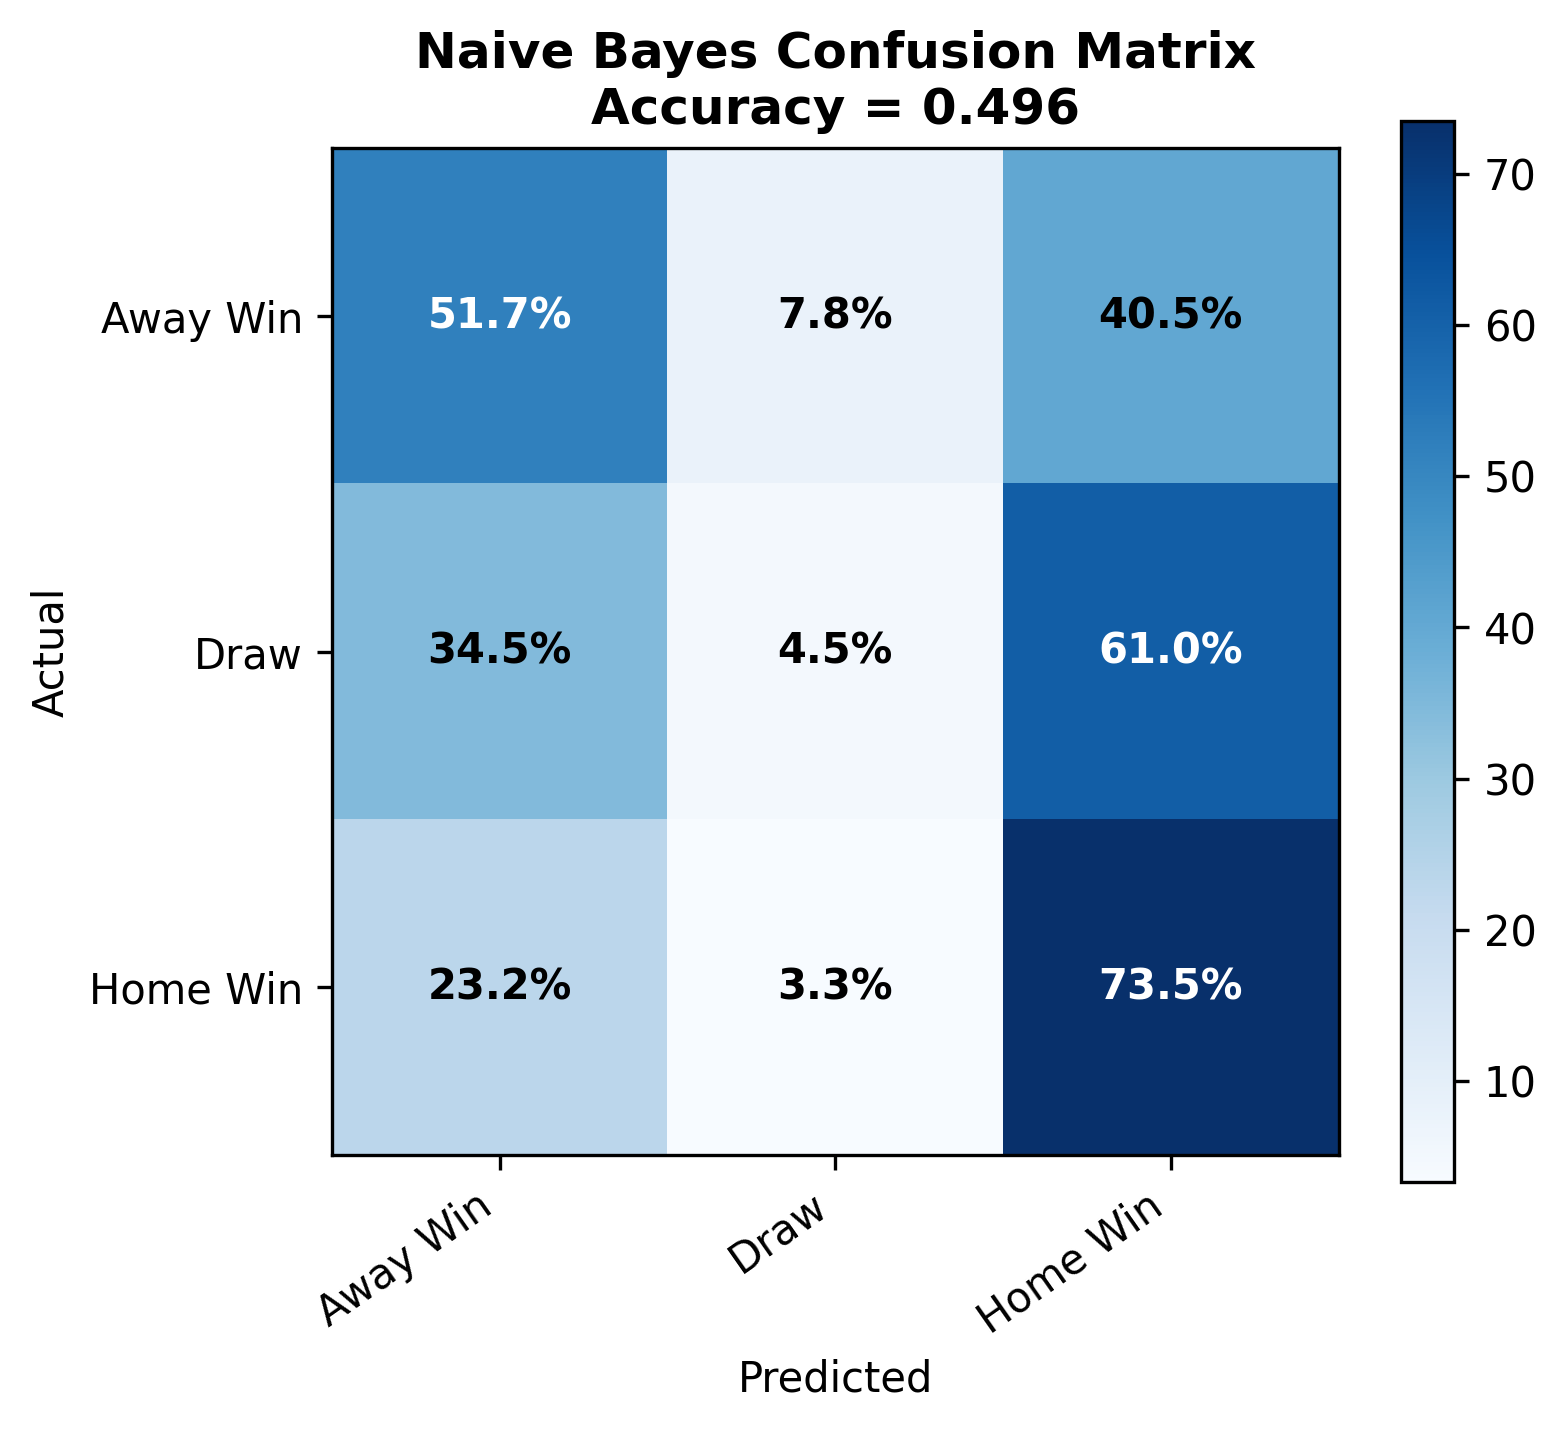
\includegraphics[width=\linewidth]{../figures/02_confusion_matrix_naive_bayes.png}
\caption{Naive Bayes}
\end{subfigure}
\begin{subfigure}{0.48\linewidth}
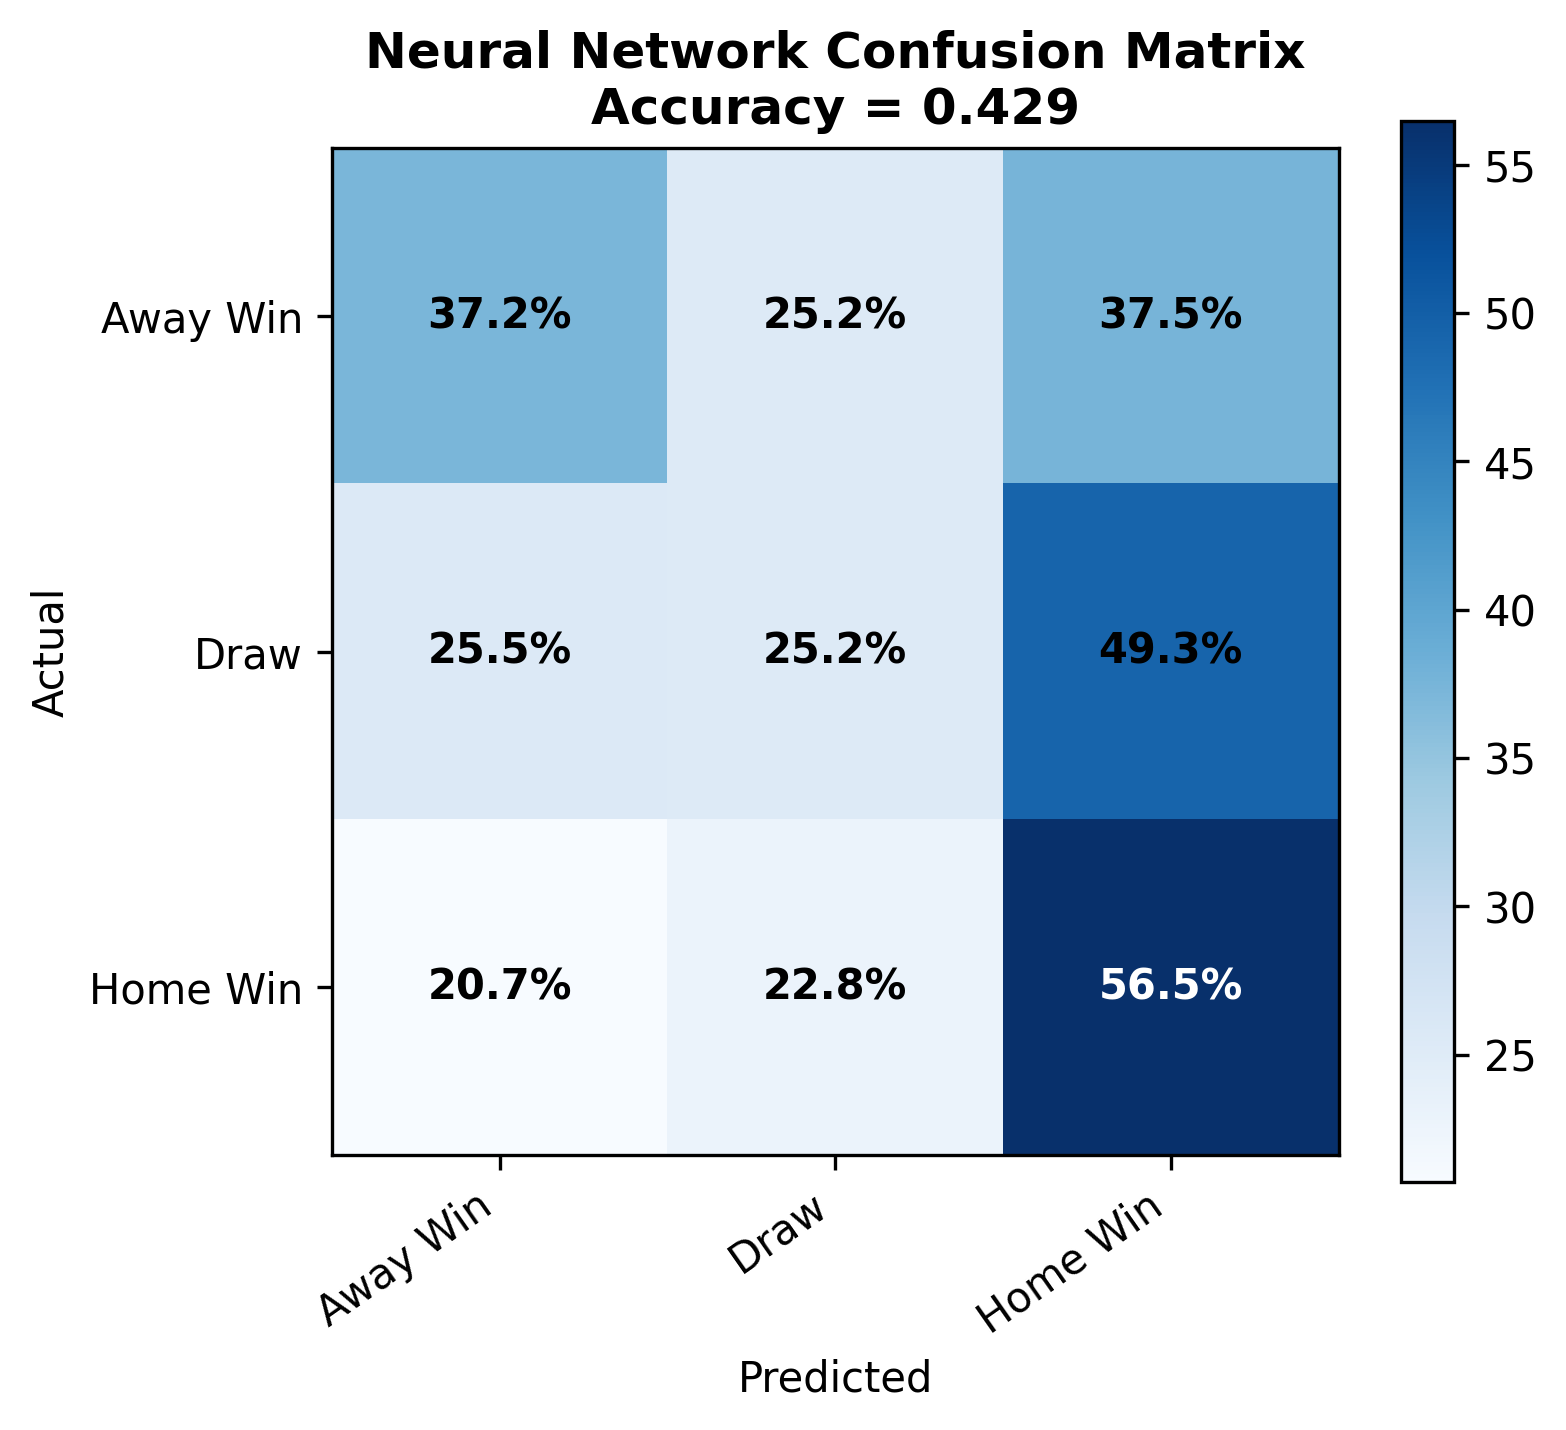
\includegraphics[width=\linewidth]{../figures/02_confusion_matrix_neural_network.png}
\caption{Neural Network}
\end{subfigure}
\caption{Confusion matrices for the remaining models.}
\end{figure}

\subsection{Class-Wise Analysis}
\begin{figure}[H]
\centering
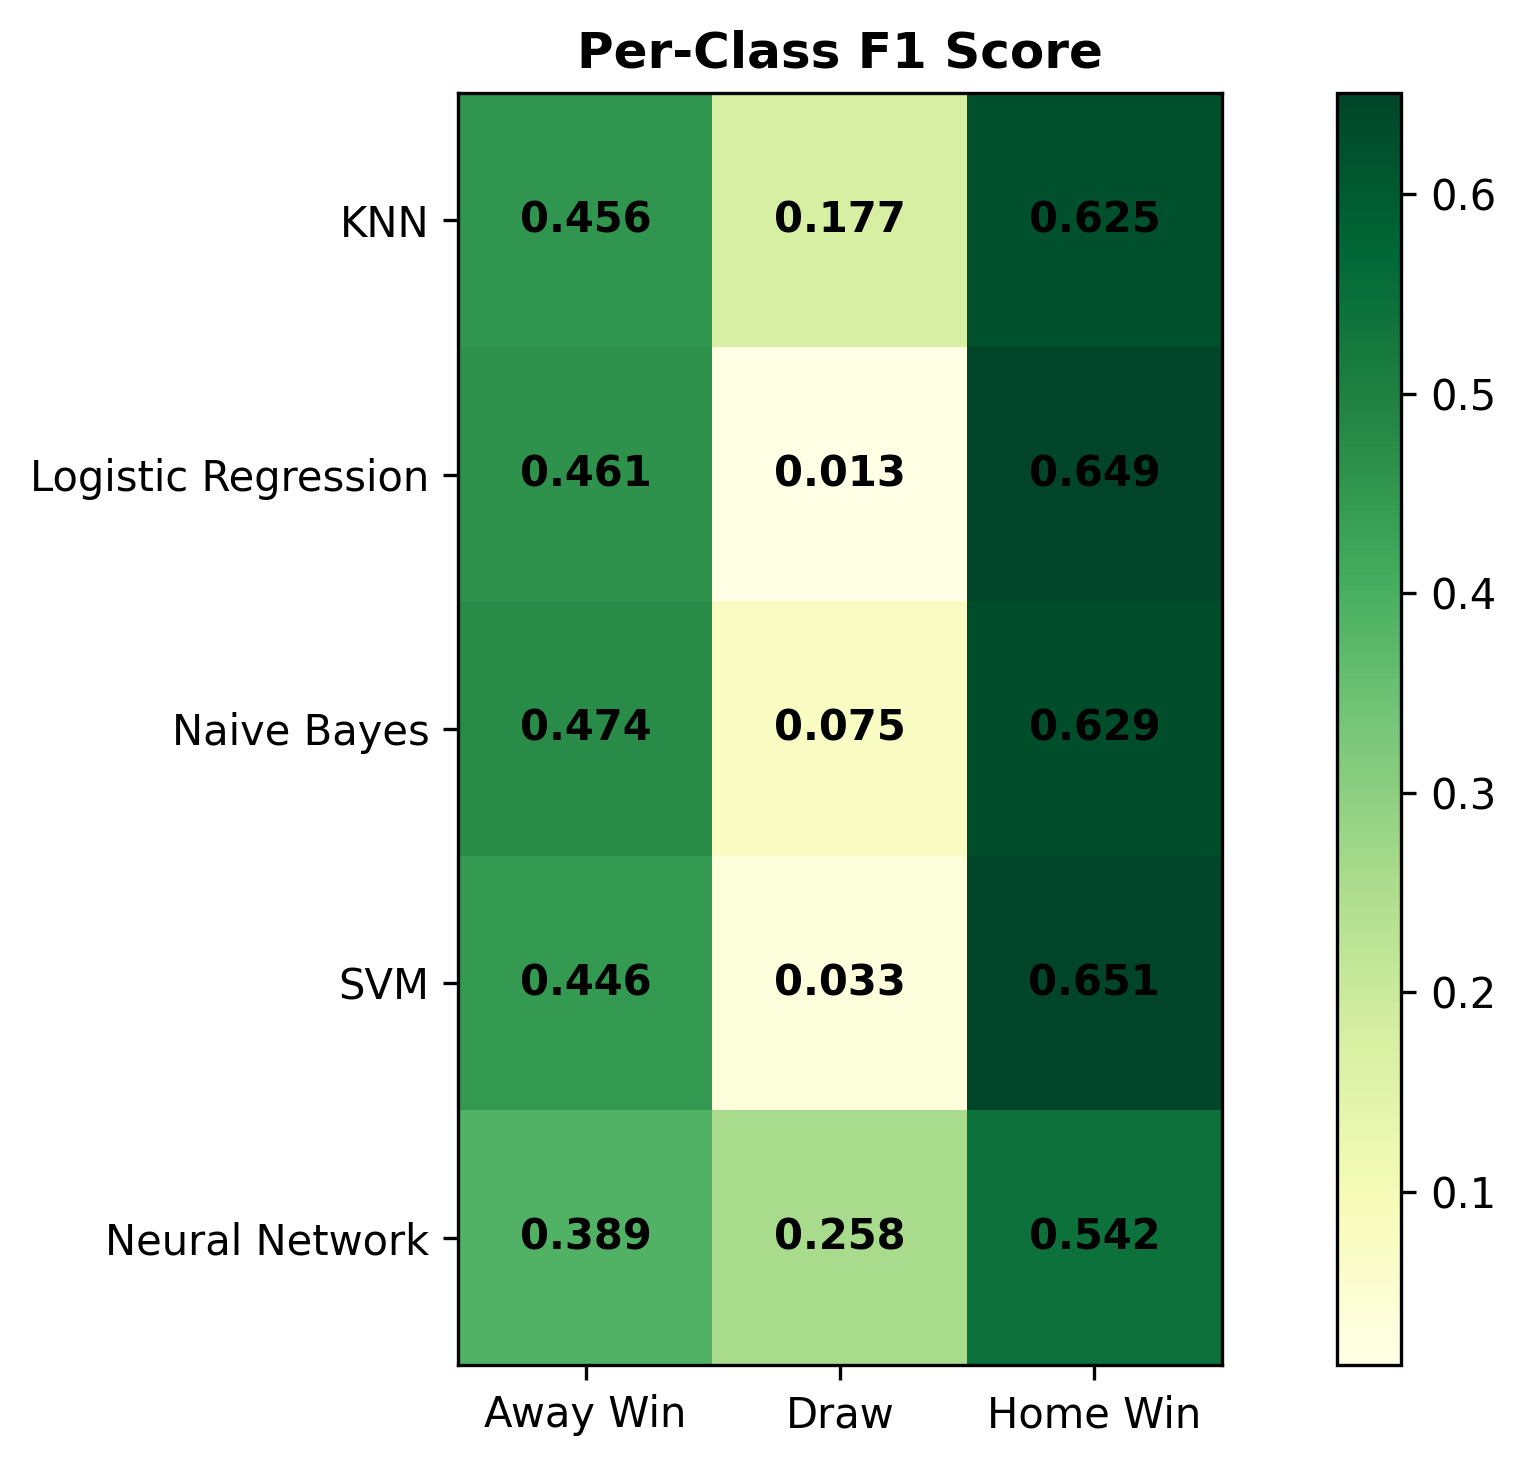
\includegraphics[width=0.65\linewidth]{../figures/03_per_class_f1.png}
\caption{Per-class F1-score heatmap.}
\end{figure}

The per-class F1-score heatmap confirms that Home Win is the easiest class to predict, while Draw is the most difficult. Neural Network predicts draws better than some other models, but its overall accuracy is lower.

\begin{figure}[H]
\centering
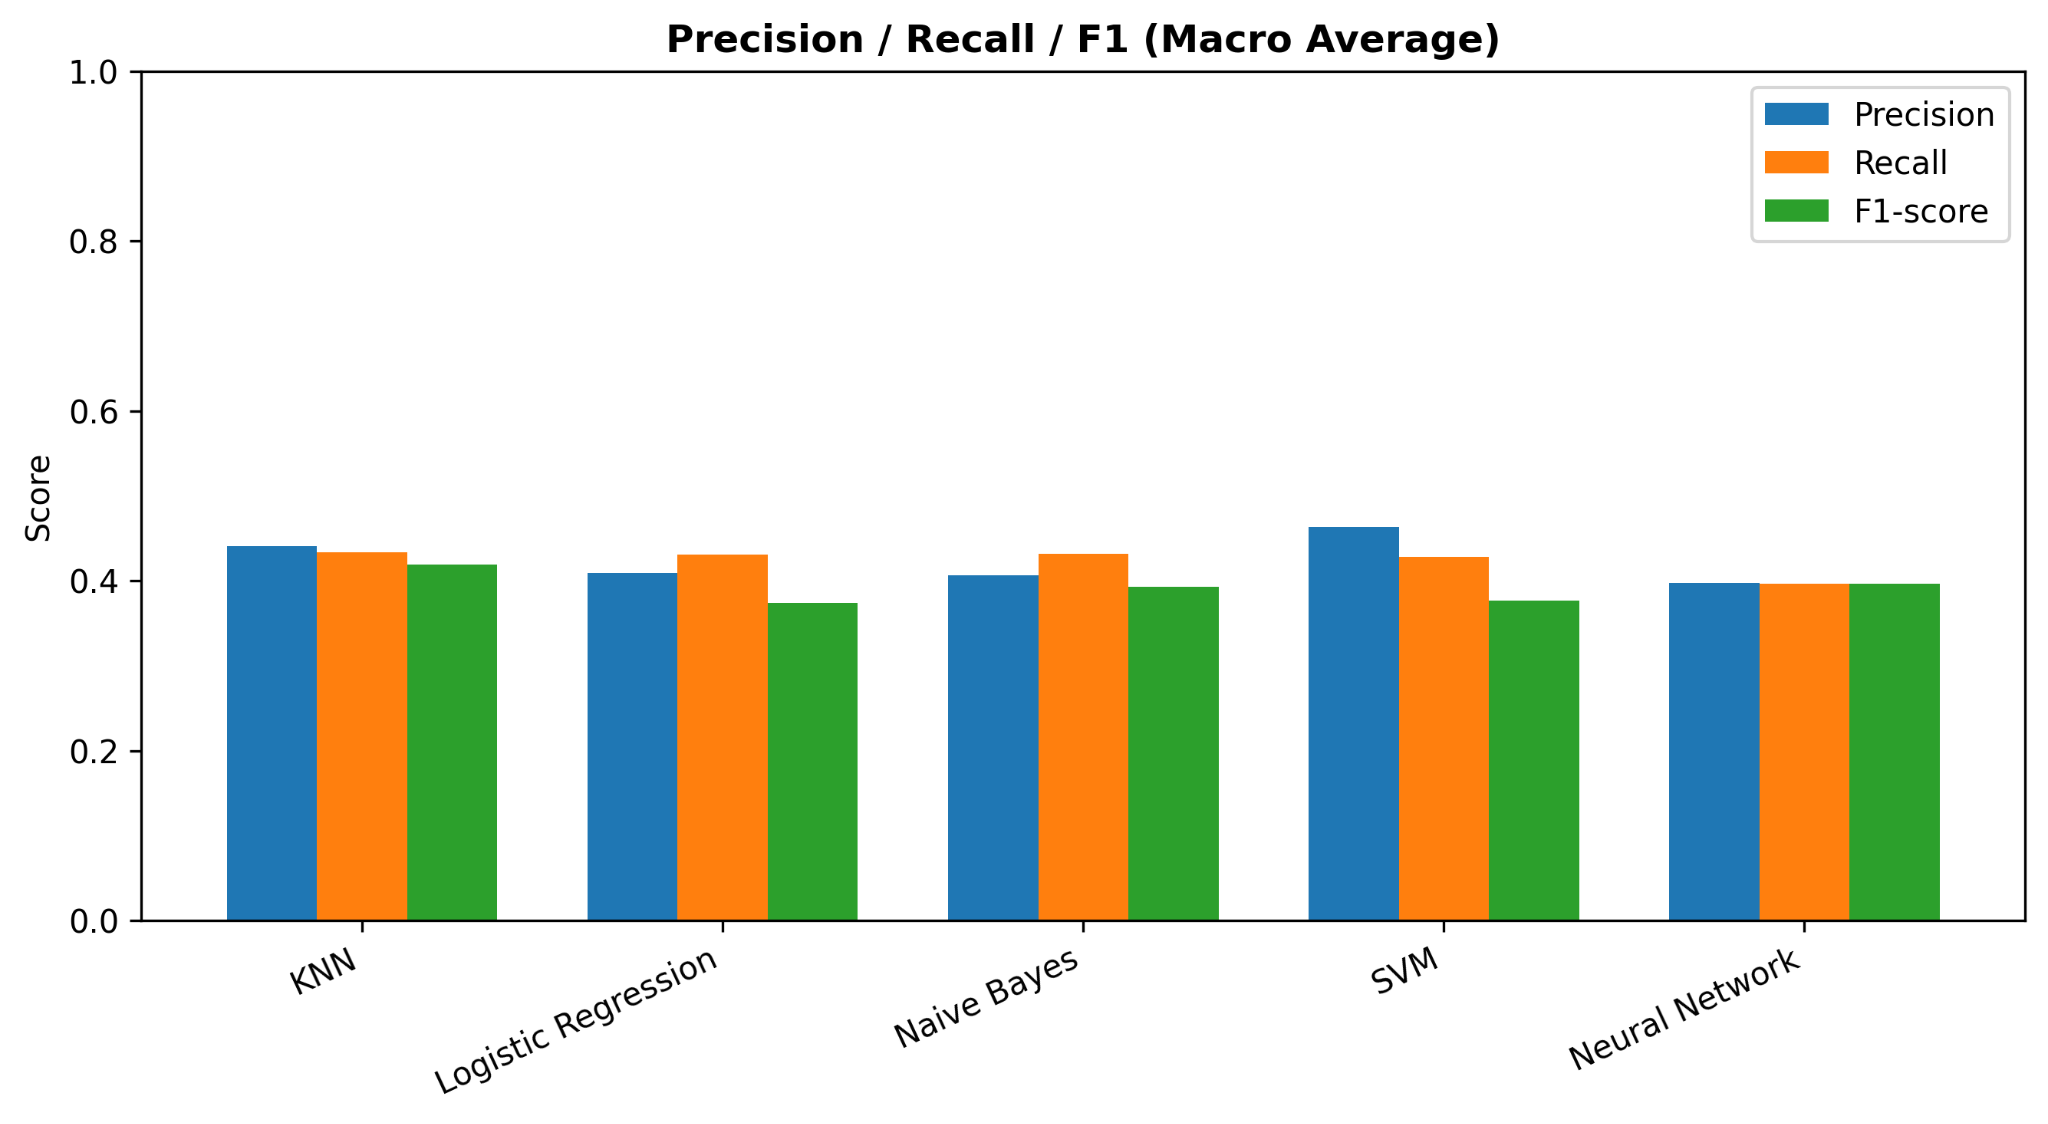
\includegraphics[width=0.82\linewidth]{../figures/04_precision_recall_f1_macro.png}
\caption{Macro precision, recall, and F1-score comparison.}
\end{figure}

\subsection{Result Distribution and Per-Season Performance}
\begin{figure}[H]
\centering
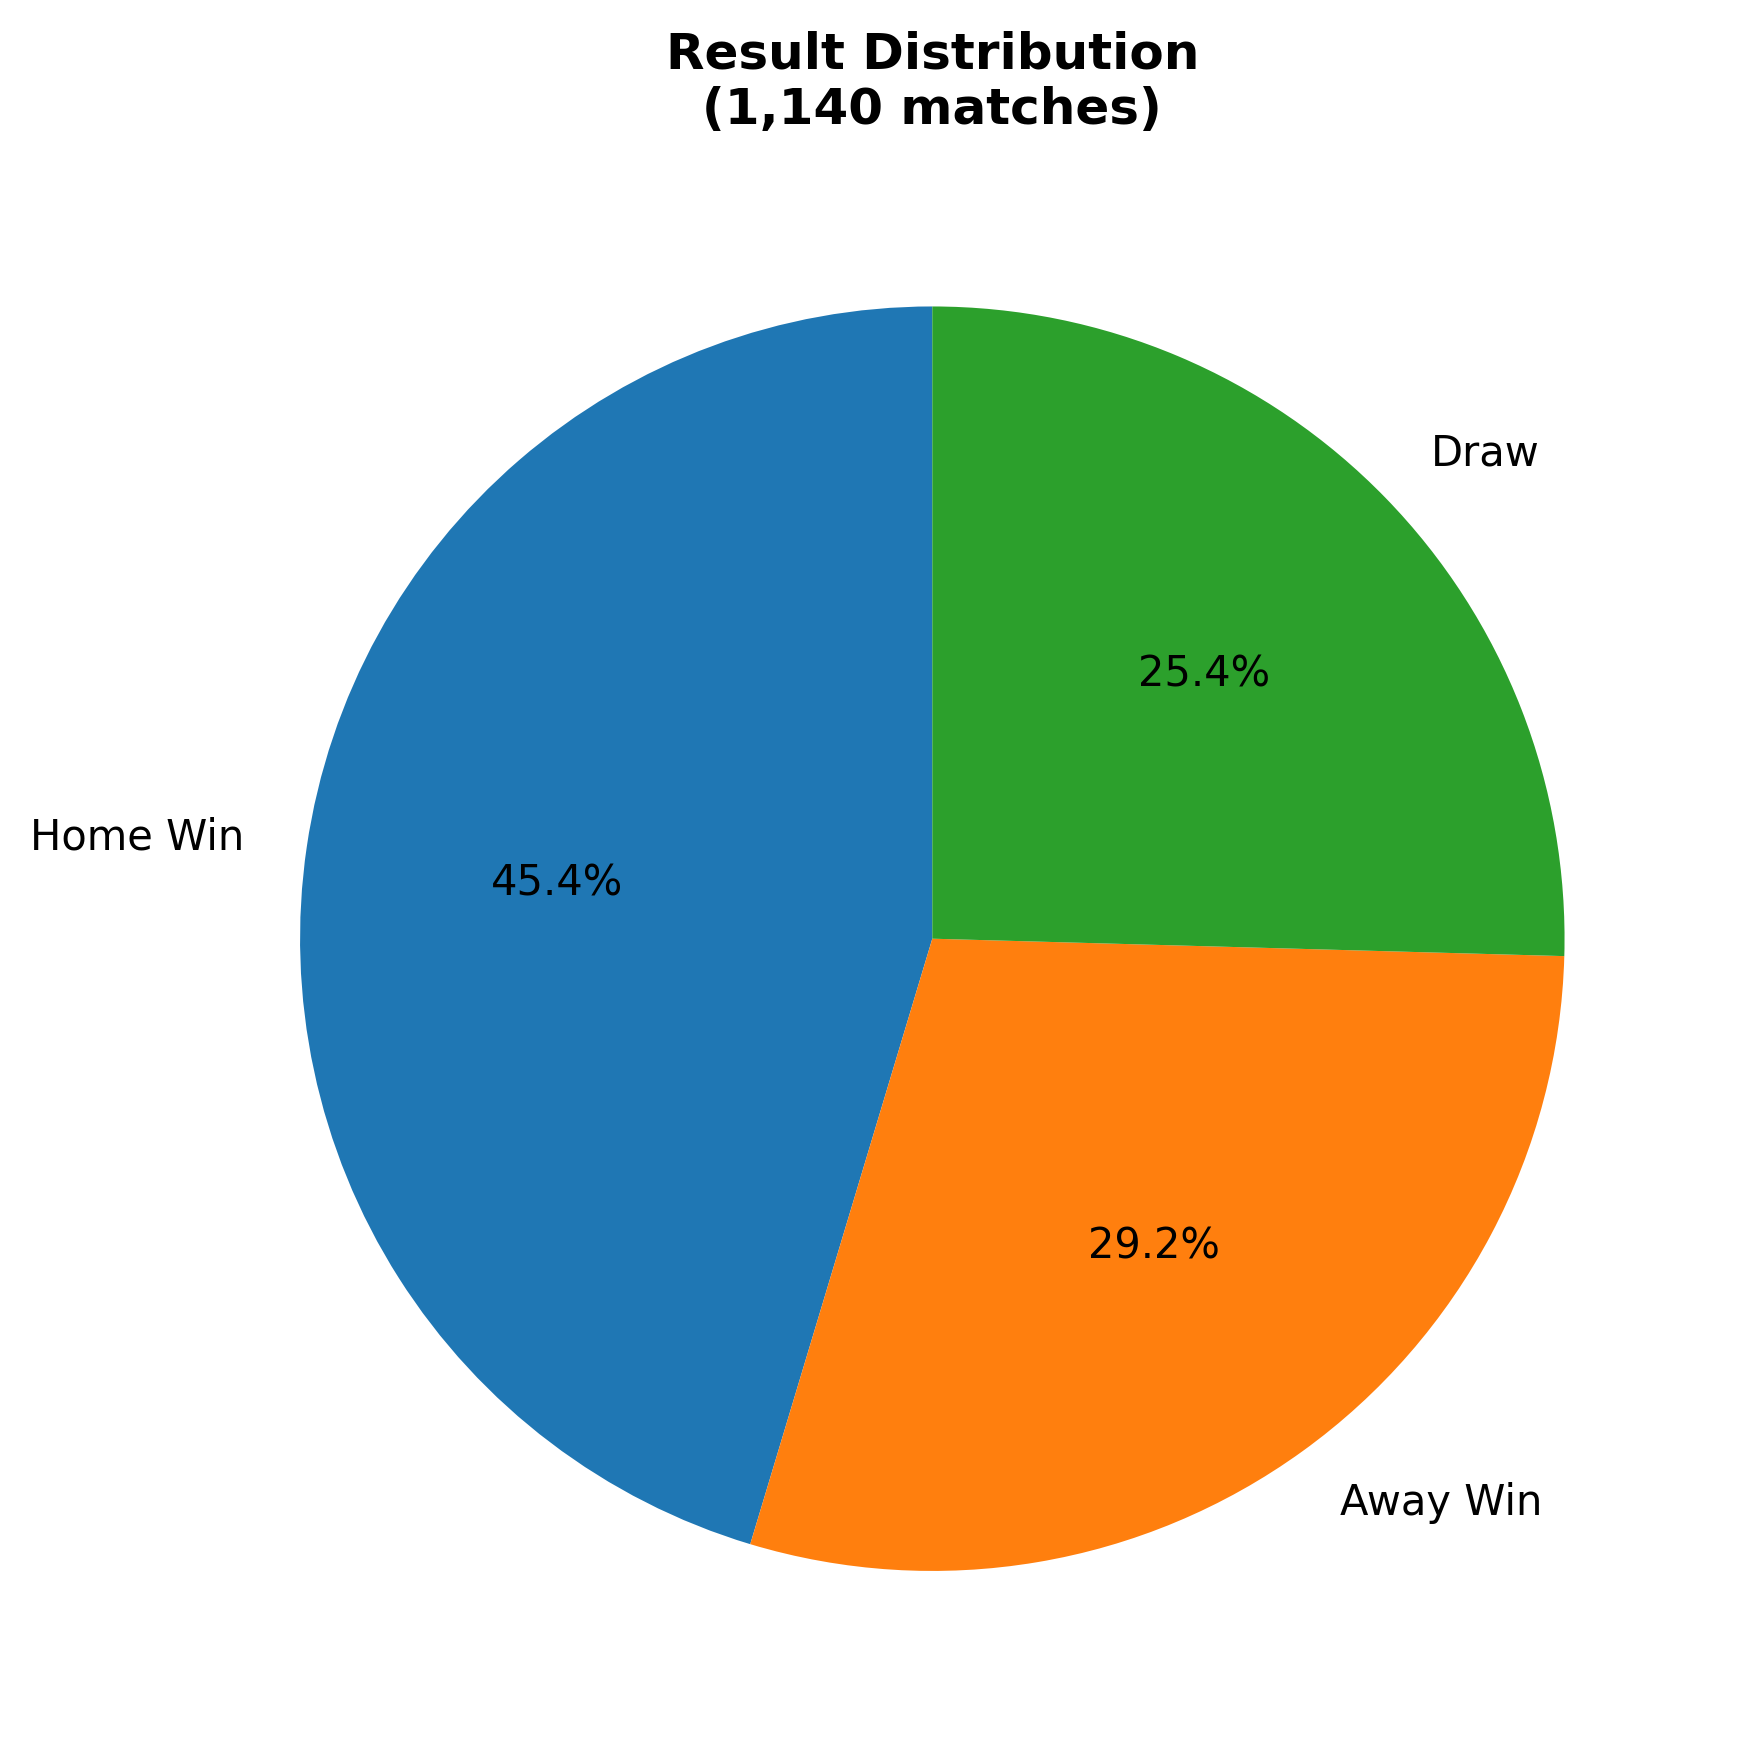
\includegraphics[width=0.55\linewidth]{../figures/05_result_distribution.png}
\caption{Class distribution of the test set.}
\end{figure}

\begin{figure}[H]
\centering
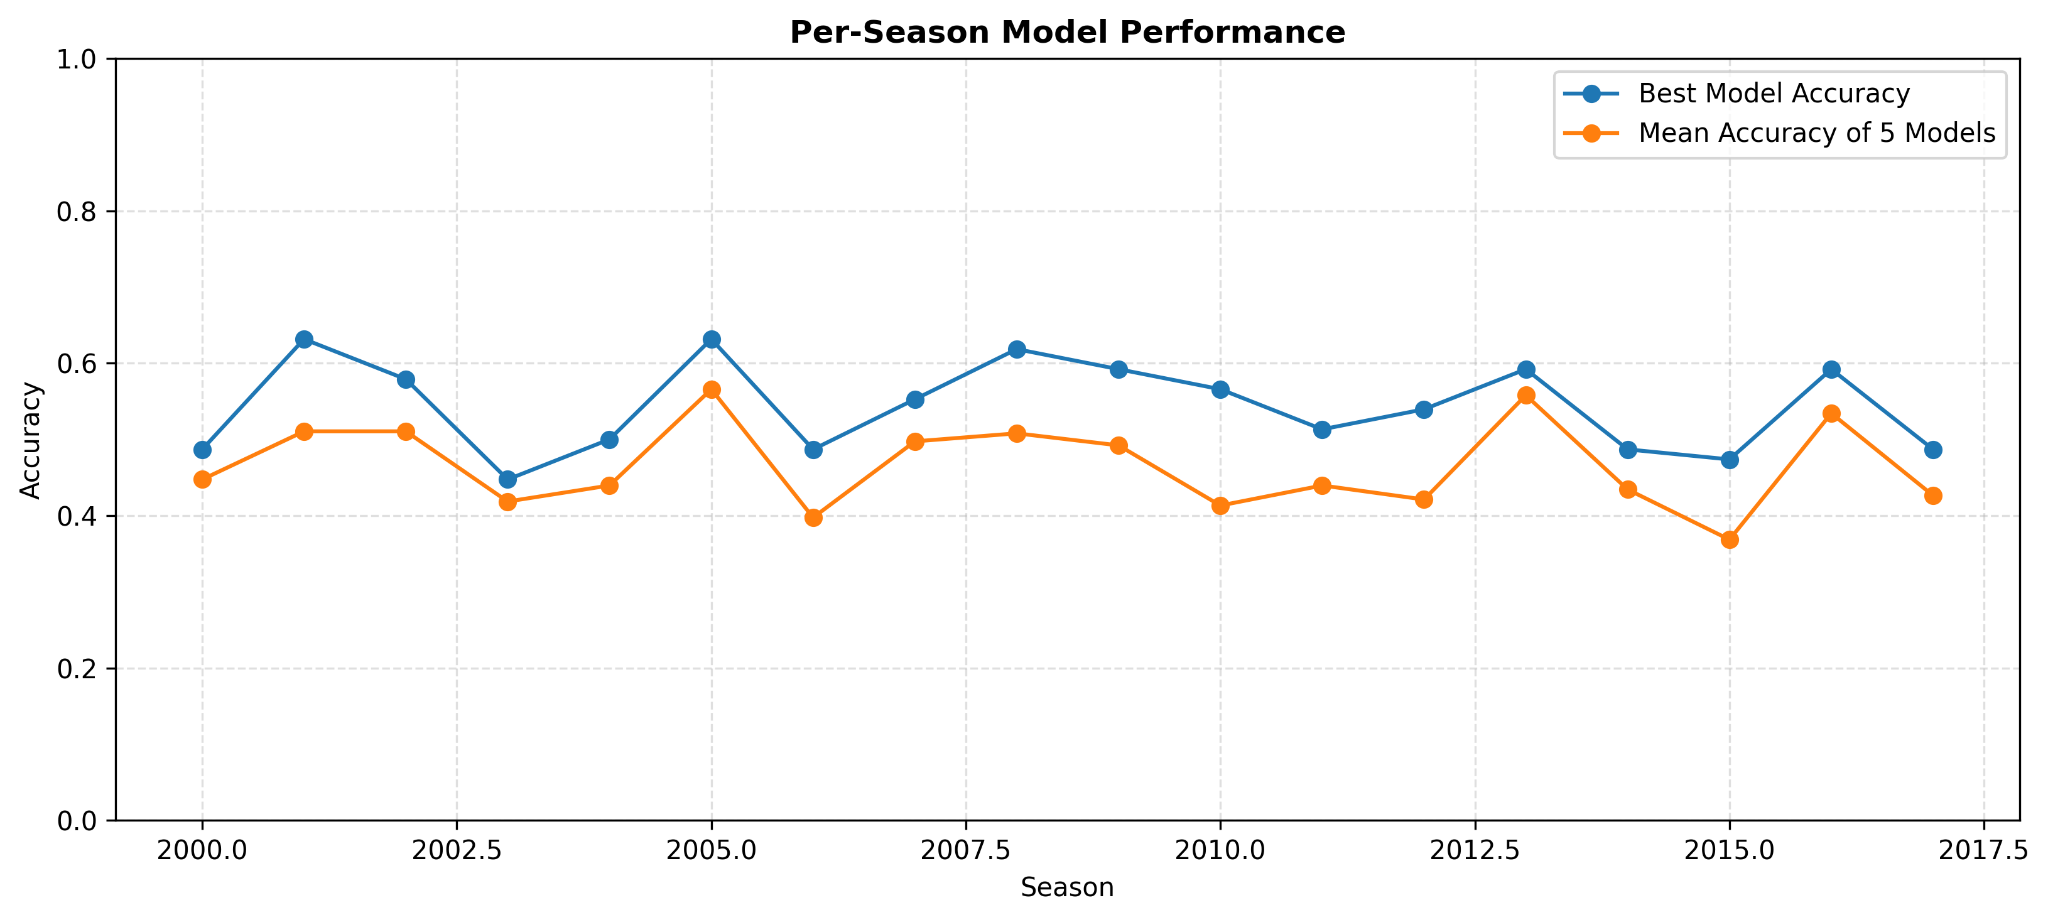
\includegraphics[width=0.90\linewidth]{../figures/06_per_season_accuracy.png}
\caption{Per-season best-model accuracy and mean accuracy of five models.}
\end{figure}

The test set contains more Home Wins than Draws, which explains why models often lean toward Home Win predictions. Per-season results show that the best model changes across seasons, indicating cross-season distribution shift.

\section{Conclusions and Future Work}
This project implemented five supervised machine learning classifiers for EPL match outcome prediction. Among the trained classifiers, SVM achieved the best accuracy of 51.58\%, while Bet365 odds achieved 54.56\% accuracy as a test-only benchmark. The results show that machine learning can provide useful predictive performance, but draw prediction remains difficult.

Future work may include adding player-level features, injury data, expected goals (xG), team market value, manager changes, ensemble models, class balancing techniques, and probability calibration. These improvements may reduce the bias toward Home Win and improve draw prediction.

\section{References}
\begin{enumerate}
    \item Tax, N. and Joustra, Y. Predicting the Dutch Football Competition Using Public Data, 2015.
    \item James, G., Witten, D., Hastie, T., and Tibshirani, R. \textit{An Introduction to Statistical Learning}. Springer.
    \item Bishop, C. M. \textit{Pattern Recognition and Machine Learning}. Springer.
    \item Kaggle EPL Dataset, English Premier League Historical Match Data.
    \item Scikit-learn Documentation, Machine Learning in Python.
\end{enumerate}

\section{Authors' Biography and Photo}
\textbf{Muhammad Owais Saeed} is an undergraduate Computer Science student at the University of Management and Technology. His interests include Machine Learning, Data Science, Artificial Intelligence, and Software Development. This project was completed for the CS446 Machine Learning course.

\vspace{0.4cm}
\noindent\fbox{\parbox[c][3cm][c]{3cm}{\centering Insert author photo here}}

\end{document}
